\chapter{Printing and Assembly}
\label{ch:printingandassembly}

\section{Printing}
\label{sec:printing}

In this section, we will describe the printing process for the prototype. This process was carried out at the Workshop of the University of Applied Sciences Brandenburg using the printer described in Section \ref{subsec:prusa_slicer_mk3s}. The following parameters are utilized for the process.

\begin{itemize}
    \item Layer Height: 0.2 mm
    \item Infill Density: 15 \%
    \item Print Speed: 60 mm/s
    \item Supports: Everywhere
    \item Filament: PLA
\end{itemize}

Table \ref{tab:finalprintingtimeandfilament} provides information on the printing time and the weight of filament used. Additionally, Figure \ref{fig:printedparts} showcases the final printed parts after removing the support materials.


\begin{table}[!ht]
    \centering
    \begin{tabular}{|l|c|c|}
        \hline
        \textbf{Part Name} & \textbf{Weight of PLA used (g)} & \textbf{Printing Time (h)} \\ \hline
        Top Cover          & 57.71                           & 2.00                       \\ \hline
        Main Body          & 245.14                          & 9.25                       \\ \hline
        Battery Cover      & 22.21                           & 0.67                       \\ \hline
        Switch Cover       & 1.31                            & 0.05                       \\ \hline
        Handle Pistol      & 64.63                           & 1.98                       \\ \hline
    \end{tabular}
    \caption{Printing Time and Filament Used}
    \label{tab:finalprintingtimeandfilament}
\end{table}

\begin{figure}[h!]
    \centering
    \begin{subfigure}[c]{0.45\textwidth}
        \begin{minipage}{\textwidth}
            \centering
            \includegraphics[height=4 cm]{texs/Part1/chapter5/image/res_main.jpg}
        \end{minipage}
        \caption{Main Body}
        \label{fig:printed_main_body}
    \end{subfigure}
    \begin{subfigure}[c]{0.45\textwidth}
        \begin{minipage}{\textwidth}
            \centering
            \includegraphics[height=4 cm]{texs/Part1/chapter5/image/res_top.jpg}
        \end{minipage}
        \caption{Top Cover}
        \label{fig:printed_top_cover}
    \end{subfigure}
    \begin{subfigure}[c]{0.45\textwidth}
        \begin{minipage}{\textwidth}
            \centering
            \includegraphics[height=4 cm]{texs/Part1/chapter5/image/res_batt.jpg}
        \end{minipage}
        \caption{Battery Cover}
        \label{fig:printed_battery_cover}
    \end{subfigure}
    \begin{subfigure}[c]{0.45\textwidth}
        \begin{minipage}{\textwidth}
            \centering
            \includegraphics[height=4 cm]{texs/Part1/chapter5/image/res_switch.jpg}
        \end{minipage}
        \caption{Switch Cover}
        \label{fig:printed_switch_cover}
    \end{subfigure}
    \begin{subfigure}[c]{0.45\textwidth}
        \begin{minipage}{\textwidth}
            \centering
            \includegraphics[height=4 cm]{texs/Part1/chapter5/image/res_grip.jpg}
        \end{minipage}
        \caption{Handle Pistol}
        \label{fig:printed_handle_pistol}
    \end{subfigure}
    \caption{Printed Parts}
    \label{fig:printedparts}
\end{figure}

\section{Assembly}
\label{sec:assembly}

The assembly process is done by following the steps below:

\subsubsection{Step 1: Installation of Threaded Inserts}
In order to securely install the brass threaded inserts into the main body, it is recommended to use a soldering iron \cite{Hermann23}. Begin by placing the chosen threaded insert onto the targeted position, aligning it with the desired hole. Heat the soldering iron to a suitable temperature, ranging from 225 $^{\circ}C$ to 245 $^{\circ}C$ for PLA material.

Once the soldering iron has reached the appropriate temperature, apply it gently to the top of the threaded insert. This process will transmit controlled heat into the material, causing the wall to soften and allow the threaded insert to be inserted. For a visual representation of how a threaded insert should look once correctly installed into the main body, please refer to Figure \ref{fig:threadedinsert}.

\begin{figure}[!ht]
    \centering
    \includegraphics[height=5cm]{texs/Part1/chapter5/image/threadinstall.jpg}
    \caption{The installed threaded insert}
    \label{fig:threadedinsert}
\end{figure}

\subsubsection{Step 2: Installation of Switch}
Installing a switch to the main body is a straightforward process that requires a few basic materials: the switch itself, a switch cover, two M2.5 nuts, and M2.5 screws. Position the switch inside the designated switch holder (see Figure \ref{fig:switchholder}), ensuring that the button faces outward for easy access.

Next, the switch cover is placed on top, aligning it with the switch and the corresponding holes in the main body. Once aligned, the M2.5 screws and nuts secure the switch and the cover to the main body. Figure \ref{fig:switchinstall} shows the completed installation of the switch.

\begin{figure}[!ht]
    \centering
    \includegraphics[height=5cm]{texs/Part1/chapter5/image/switchhole.png}
    \caption{The Switch Holder}
    \label{fig:switchholder}
\end{figure}

\begin{figure}[!ht]
    \centering
    \includegraphics[height=5cm]{texs/Part1/chapter5/image/switchinstall.jpg}
    \caption{The installed switch}
    \label{fig:switchinstall}
\end{figure}

\subsubsection{Step 3: Installation of LAN Port}

This step begins by locating the slot of the LAN port on the main body, which is located on the right side of the main body (see Figure \ref{fig:lanslot}). The LAN port is inserted into the slot and secured using the M3 screws. Figure \ref{fig:laninstall} shows the completed installation of the LAN port.

\begin{figure}[!ht]
    \centering
    \includegraphics[height=5cm]{texs/Part1/chapter5/image/lanslot.png}
    \caption{The LAN Port Slot}
    \label{fig:lanslot}
\end{figure}

\begin{figure}[!ht]
    \centering
    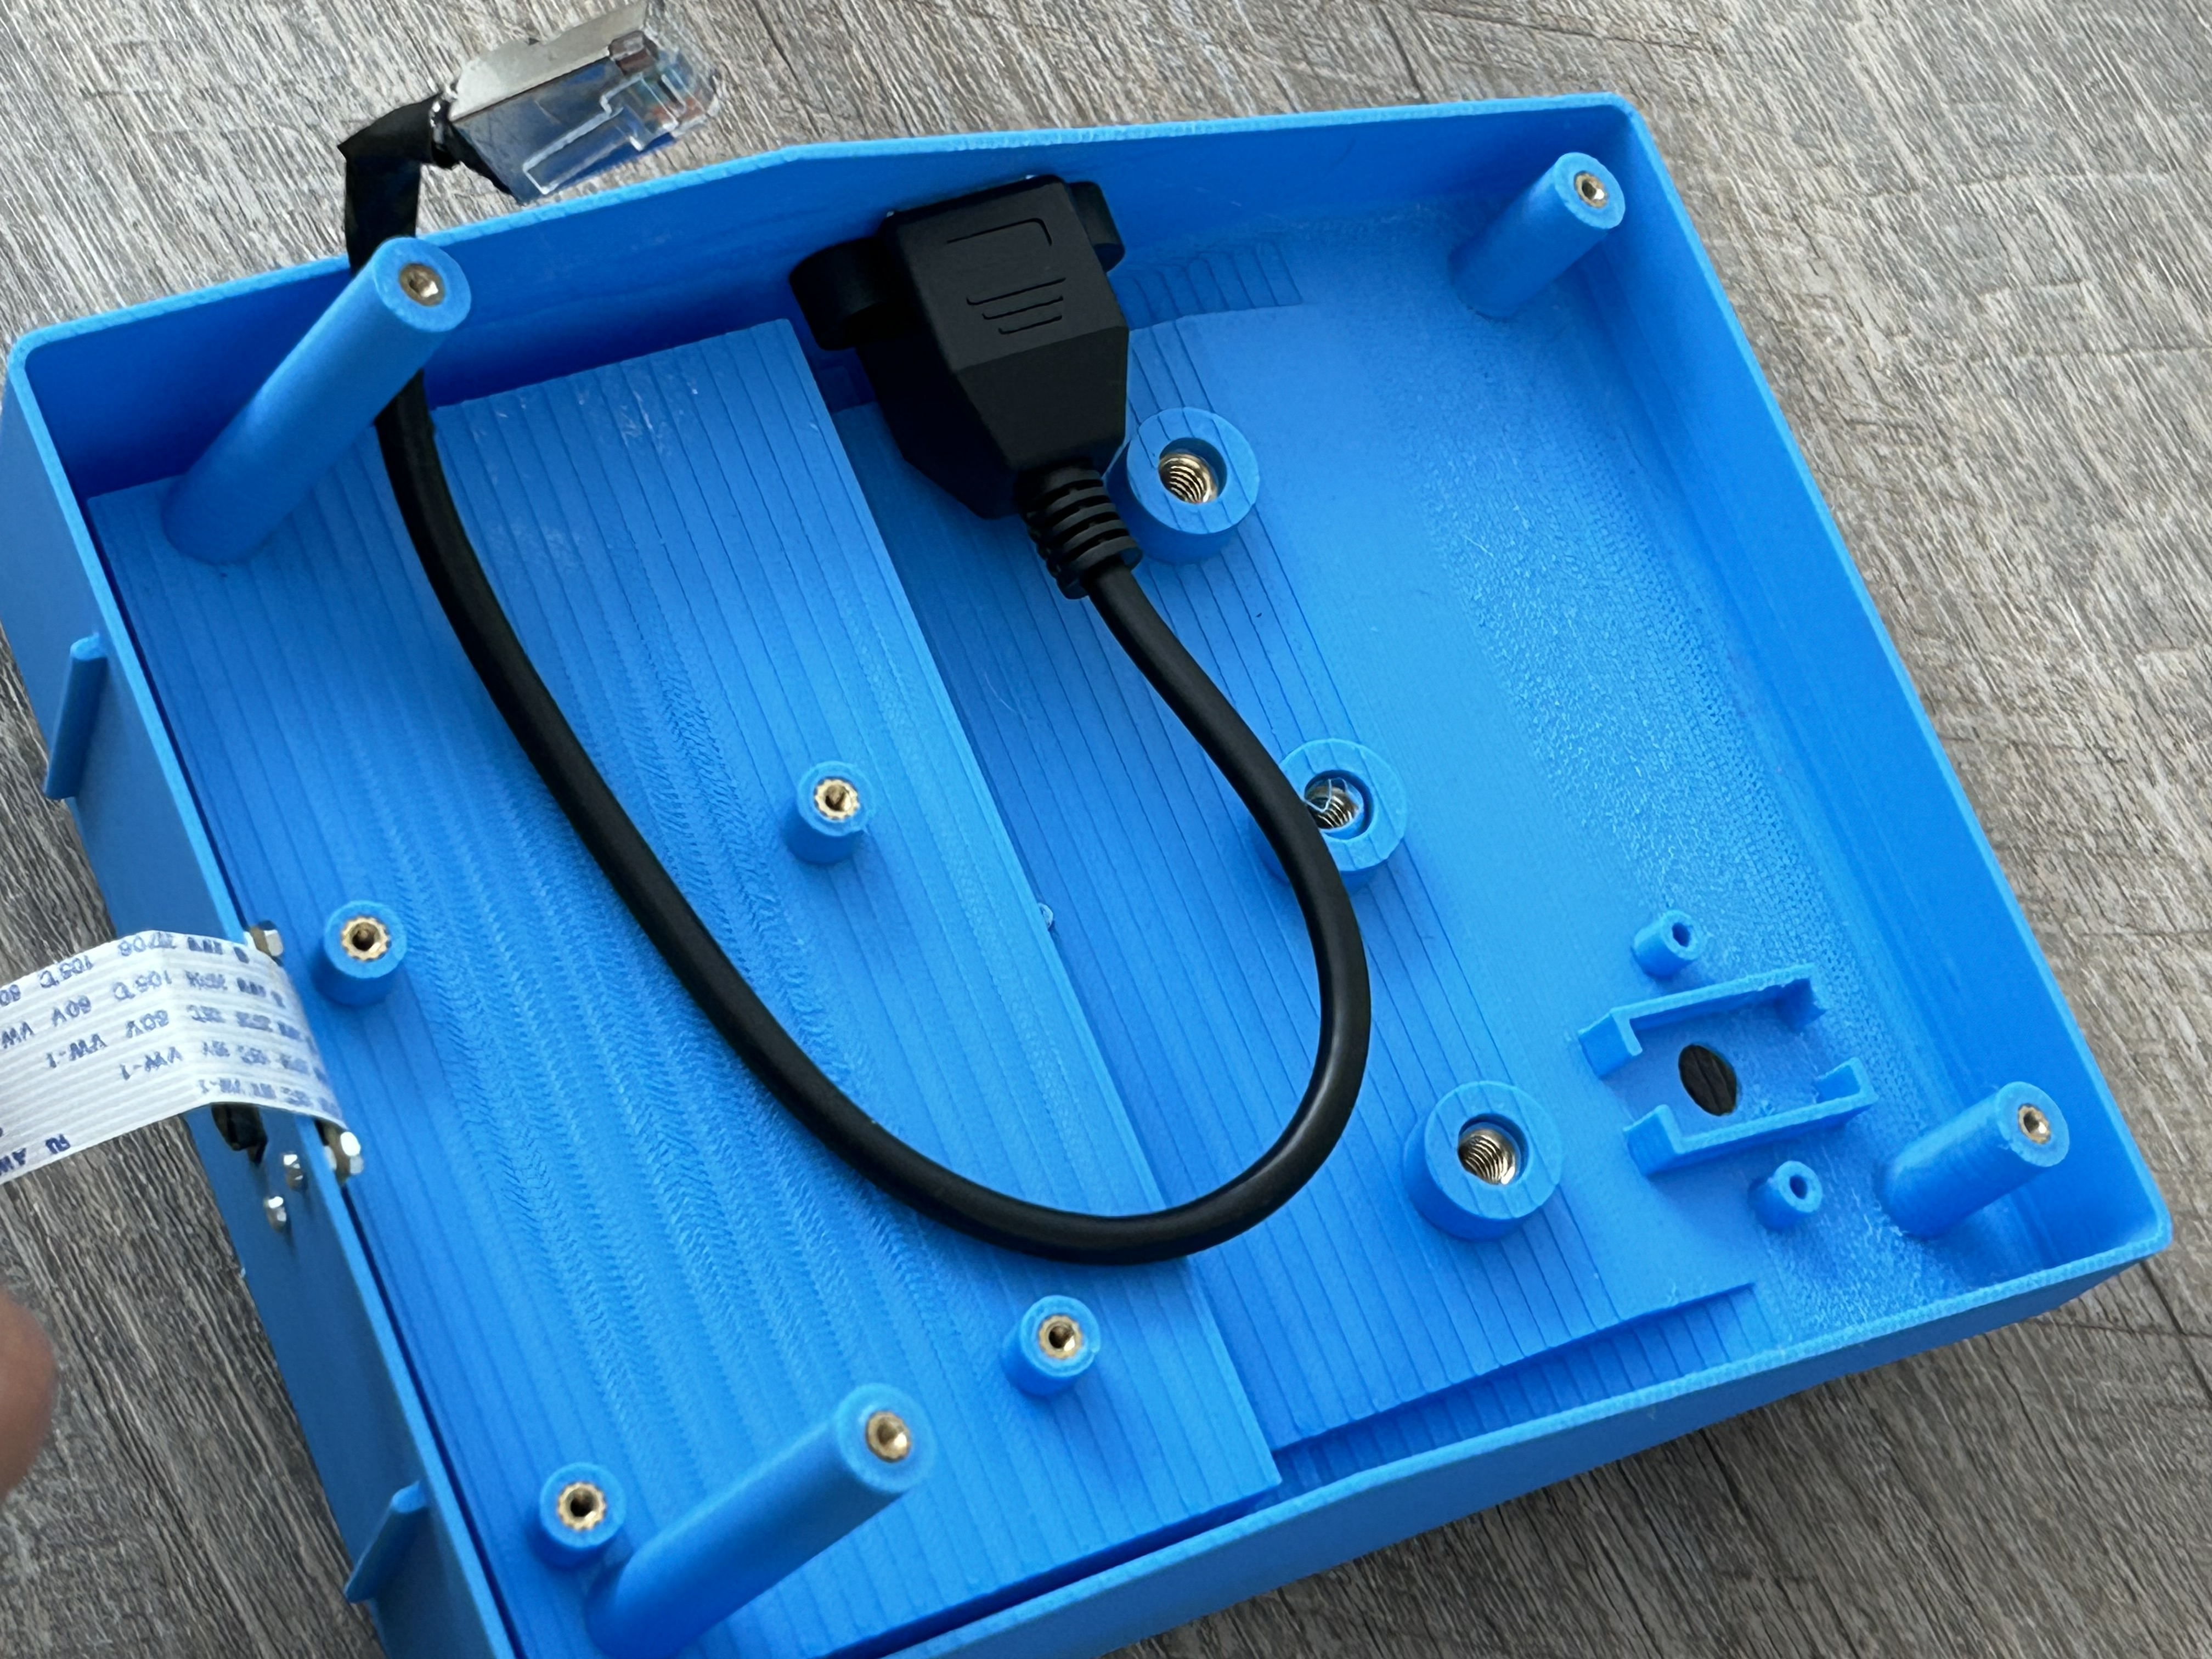
\includegraphics[height=5cm]{texs/Part1/chapter5/image/laninstall.jpg}
    \caption{The installed LAN port}
    \label{fig:laninstall}
\end{figure}

\subsubsection{Step 4: Installation of Camera Module}

The camera module is installed to the main body using M2 screws. The camera module is placed in the designated slot on the main body (see Figure \ref{fig:cameraslot}). The M2 screws are then used to secure the camera module to the main body. Figure \ref{fig:camerainstall} shows the completed installation of the camera module.

\begin{figure}[!ht]
    \centering
    \includegraphics[height=5cm]{texs/Part1/chapter5/image/camslot.png}
    \caption{The Camera Module Slot}
    \label{fig:cameraslot}
\end{figure}

\begin{figure}[!ht]
    \centering
    \includegraphics[height=5cm]{texs/Part1/chapter5/image/caminstall.jpg}
    \caption{The installed camera module}
    \label{fig:camerainstall}
\end{figure}

\subsubsection{Step 5: Installation of Battery}
To start the installation process, insert the battery into the holder as shown in Figure \ref{fig:batteryholder}. Then, connect the battery to the switch with a 90-degree USB-A to USB-C connector.

To fasten the battery to the main body, place the battery cover over the battery and main body. Use the M2.5 screws to secure the battery cover to the main body. The finished battery installation can be seen in Figure \ref{fig:batteryinstall}.

\begin{figure}[!ht]
    \centering
    \includegraphics[height=5cm]{texs/Part1/chapter5/image/battslot.png}
    \caption{The Battery Holder}
    \label{fig:batteryholder}
\end{figure}

\begin{figure}[ht!]
    \centering
    \begin{subfigure}[c]{0.45\textwidth}
        \begin{minipage}{\textwidth}
            \centering
            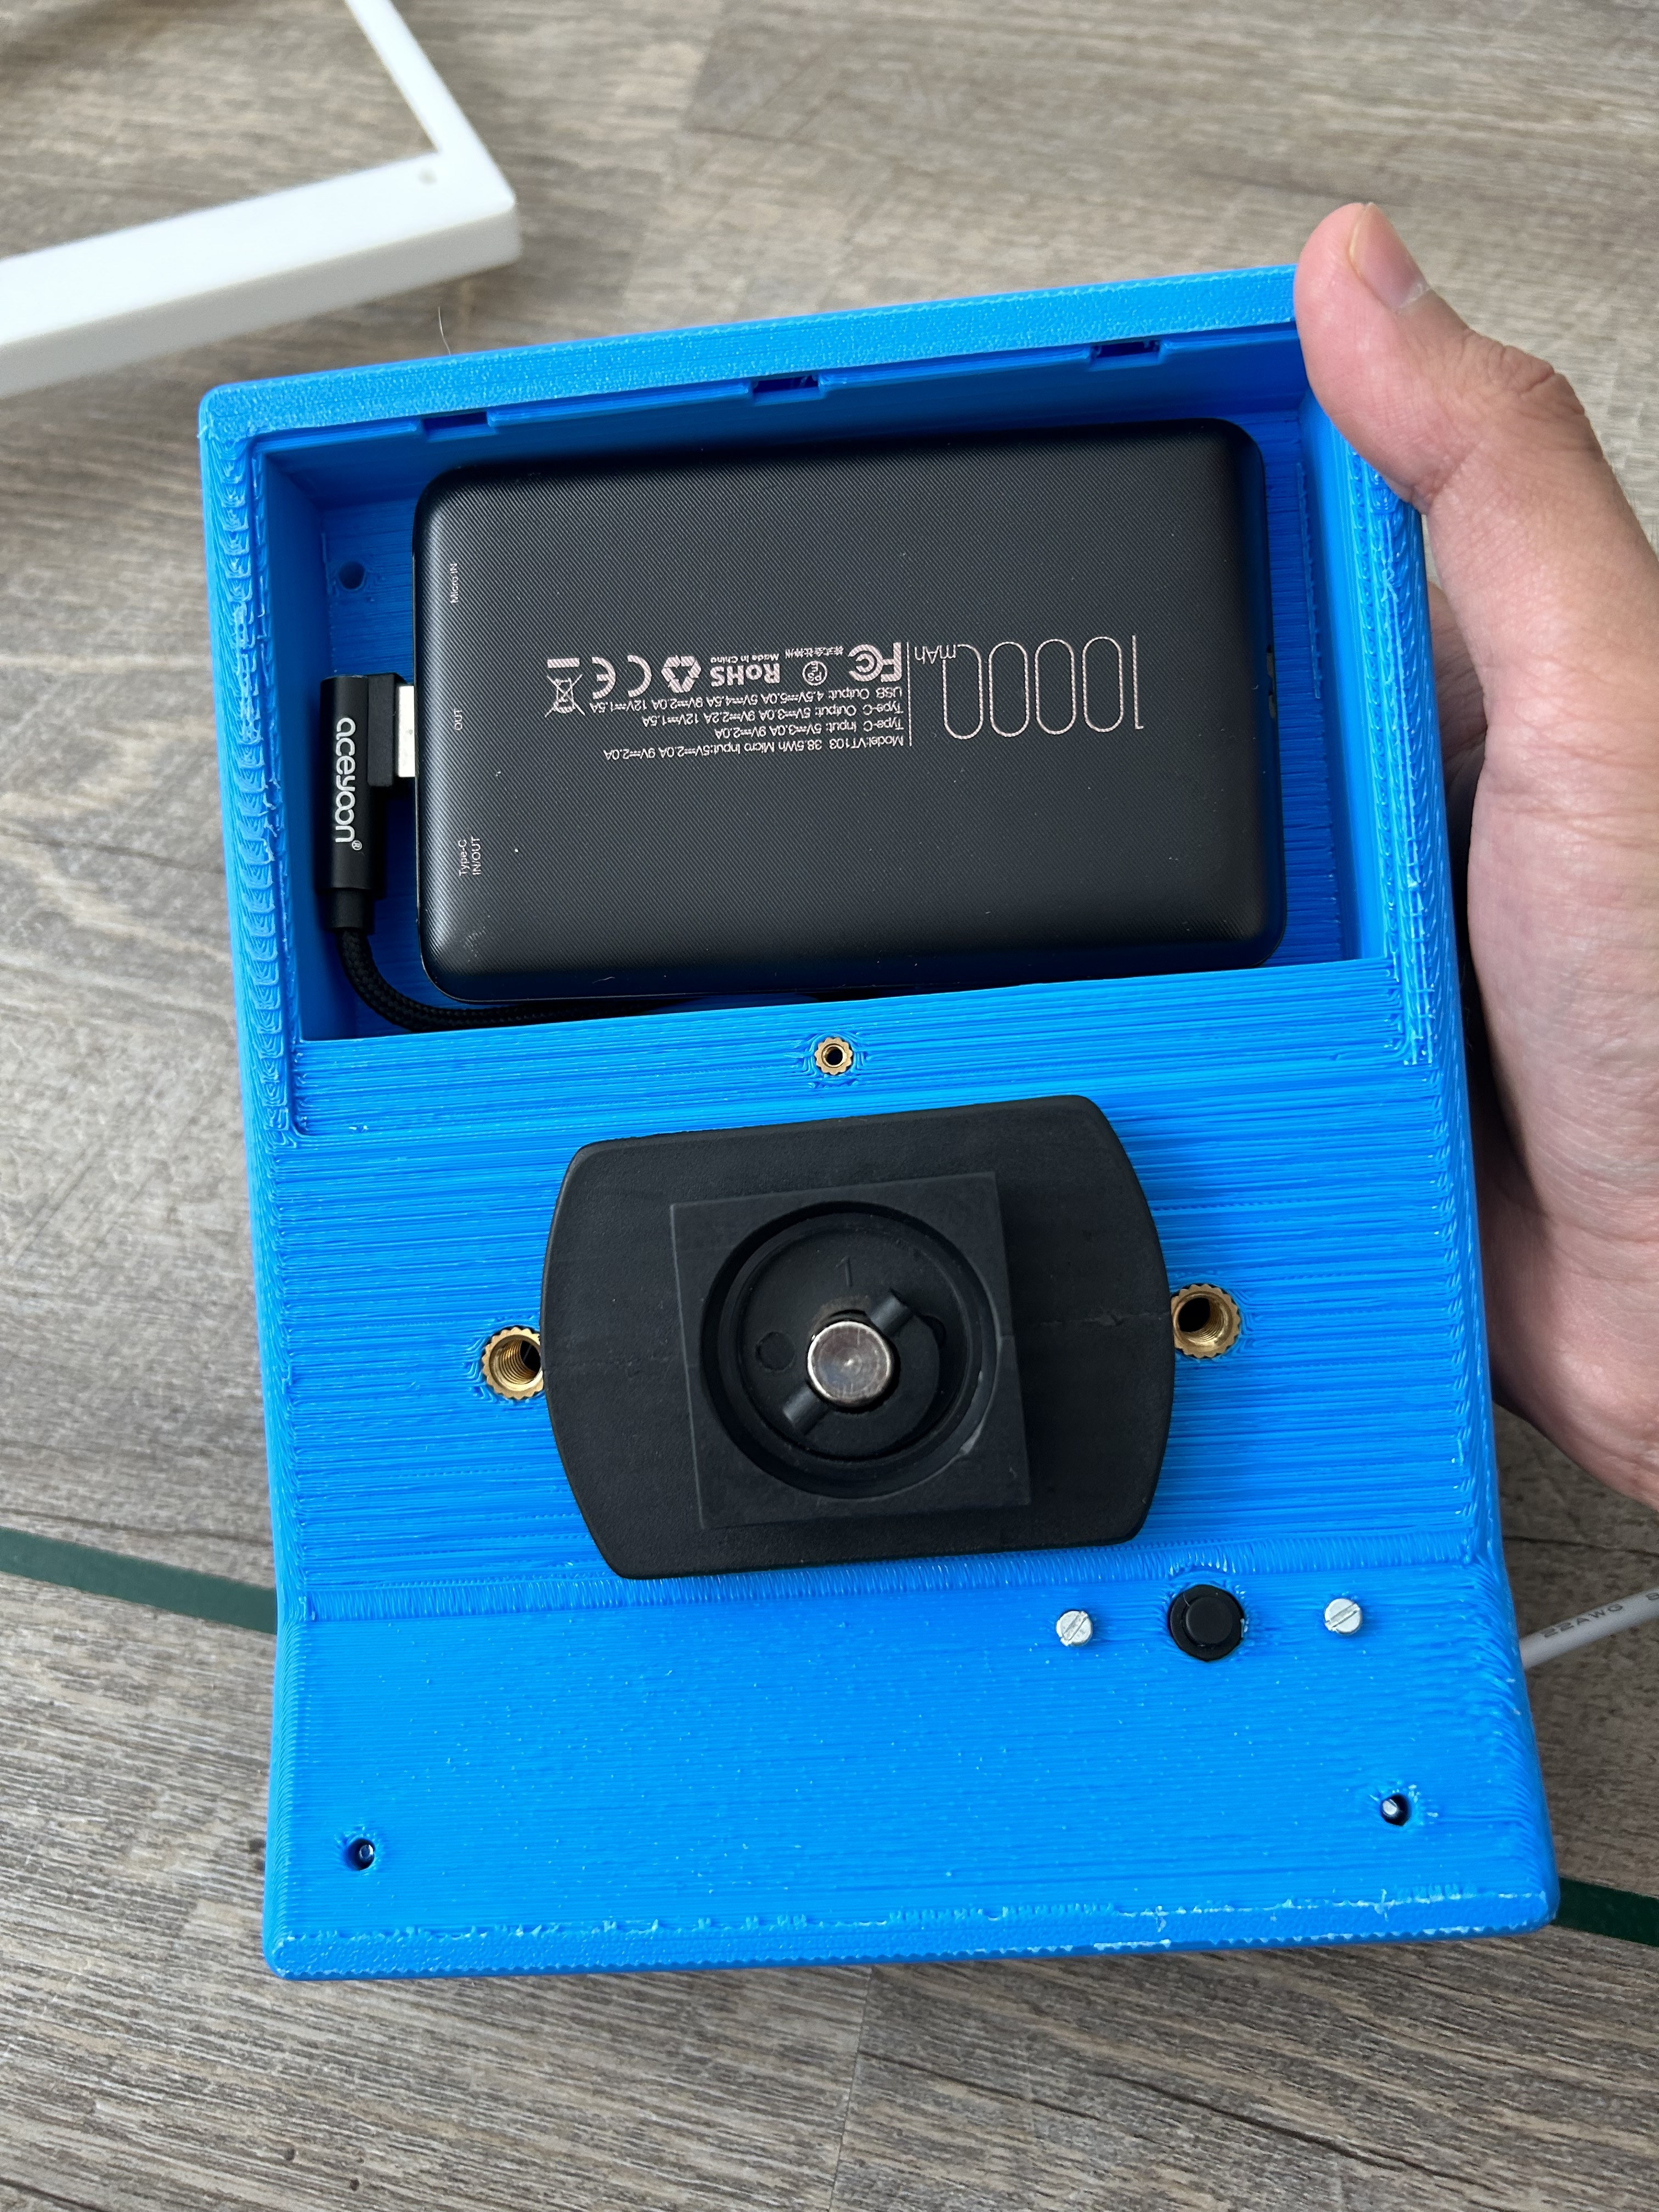
\includegraphics[height=5 cm]{texs/Part1/chapter5/image/battinstall1.jpg}
        \end{minipage}
        \caption{Without Battery Cover}
        \label{fig:battery_install_1}
    \end{subfigure}
    \begin{subfigure}[c]{0.45\textwidth}
        \begin{minipage}{\textwidth}
            \centering
            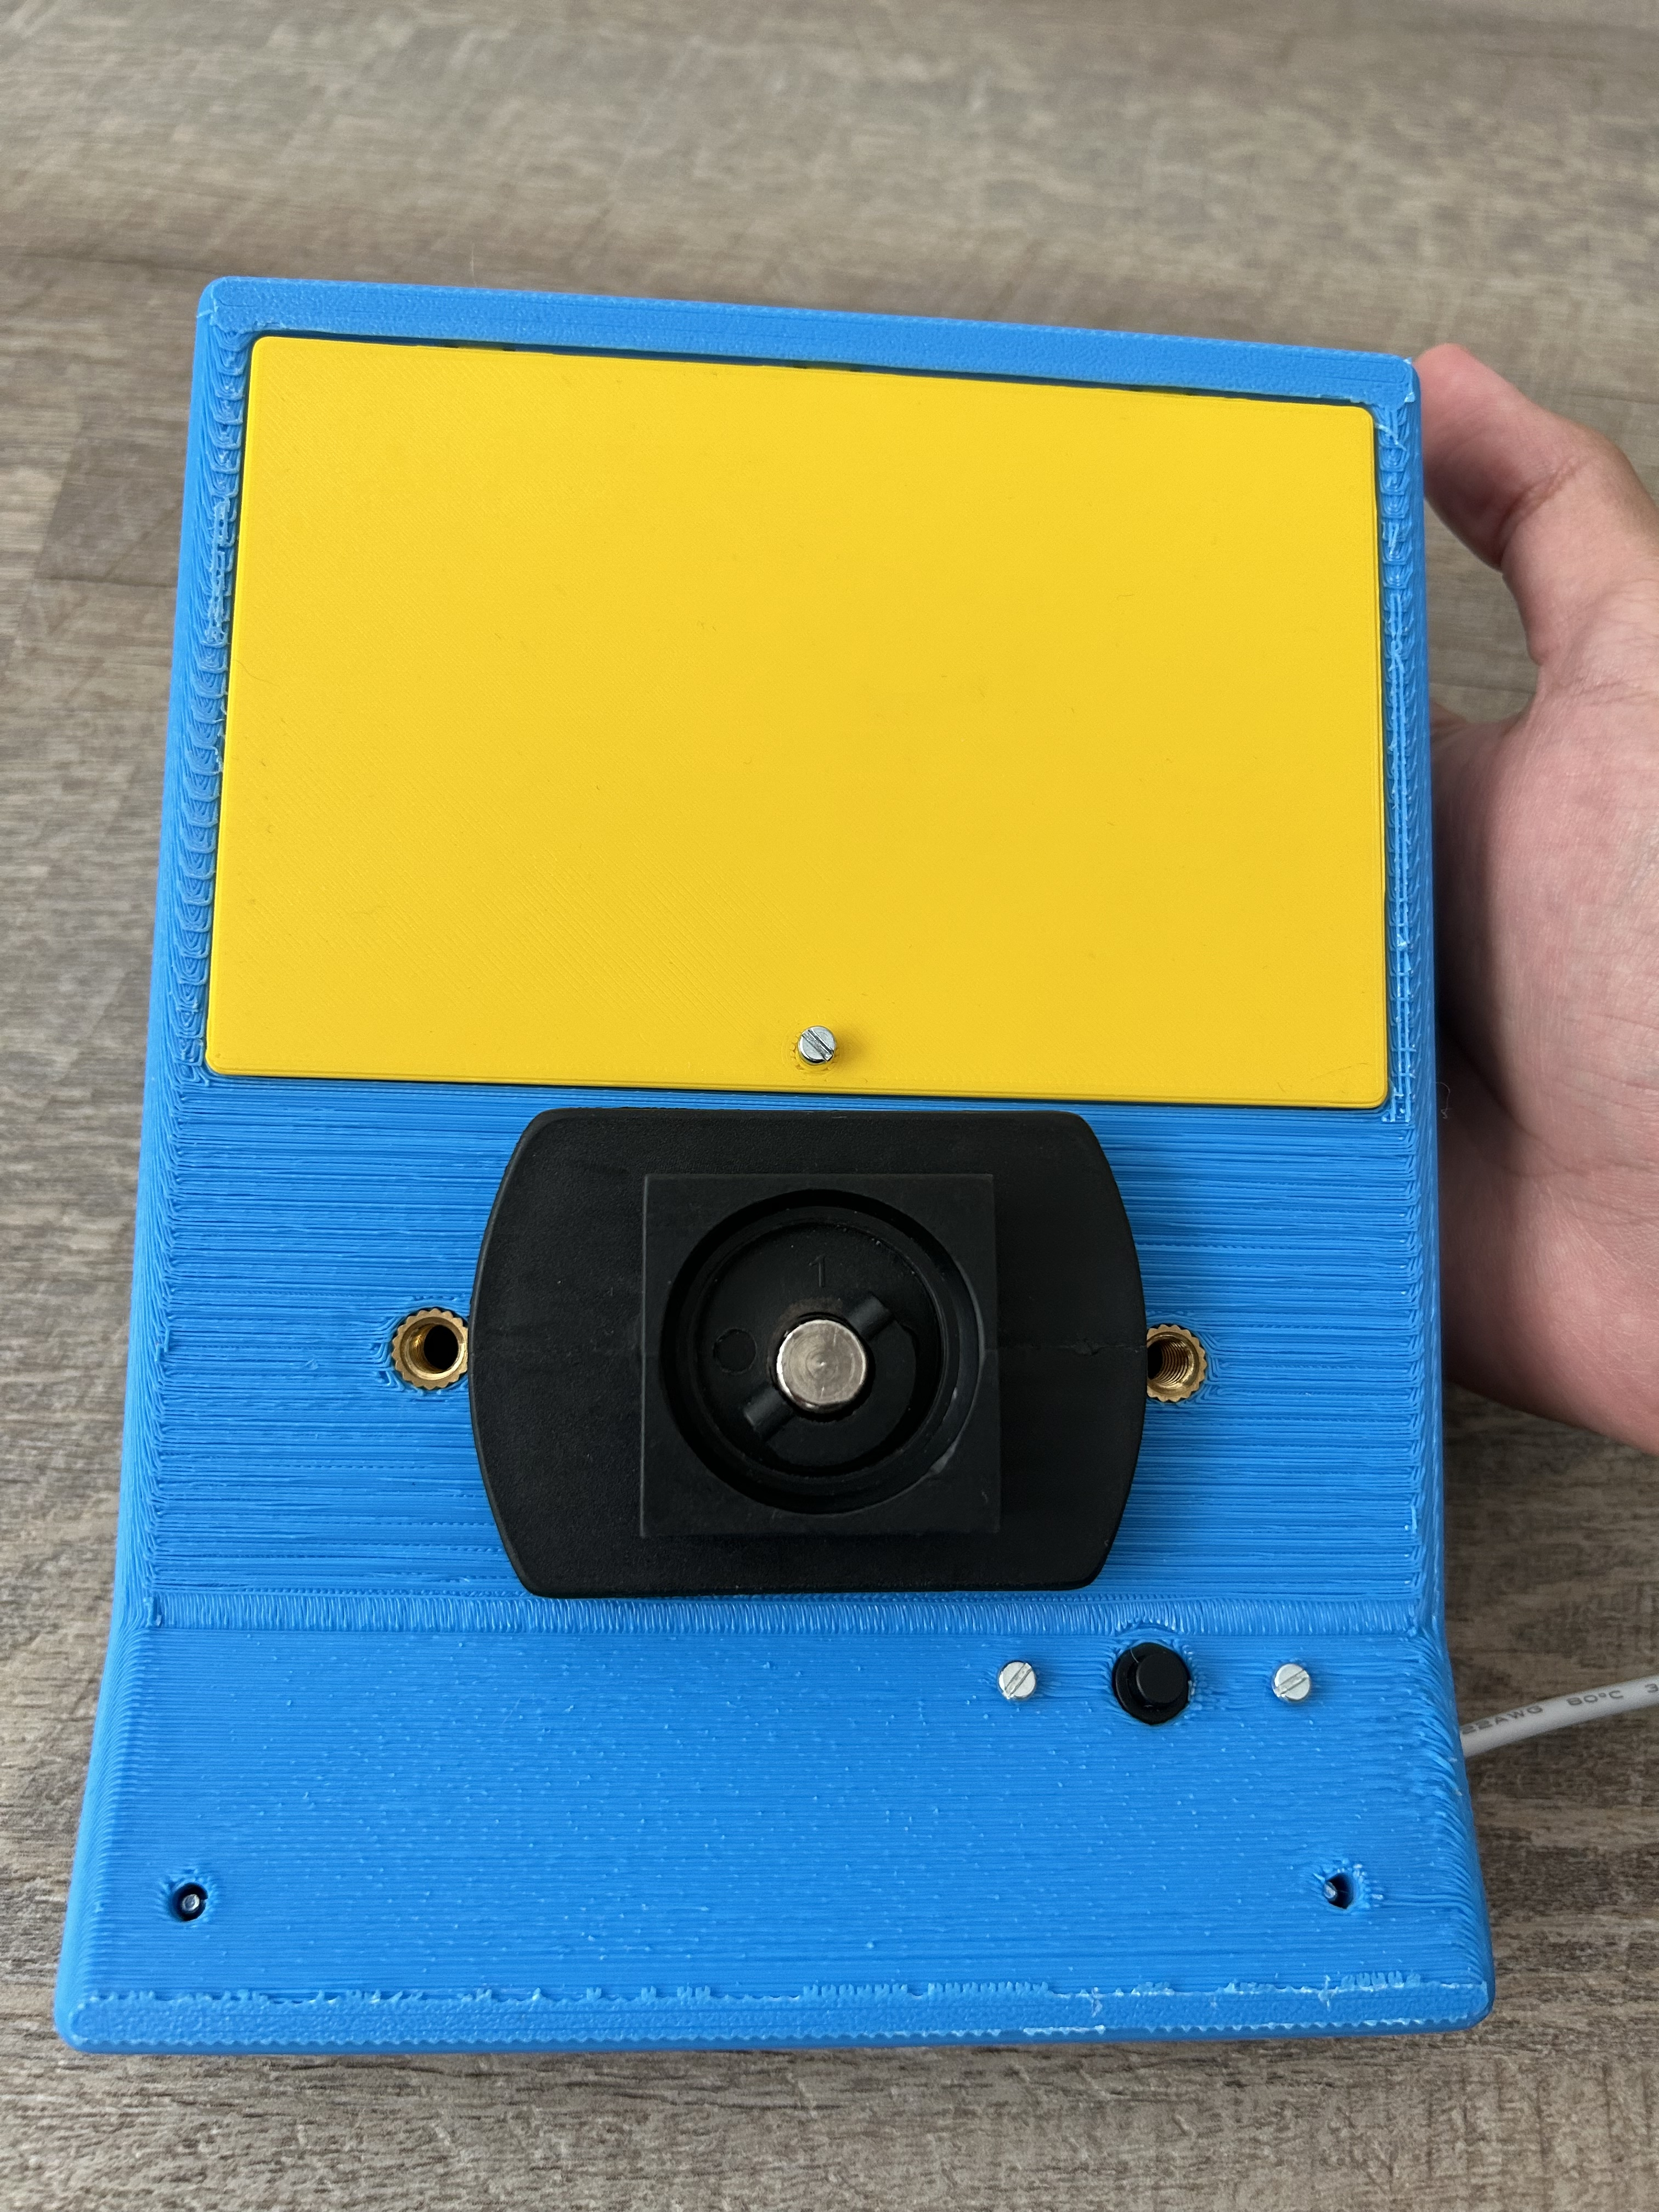
\includegraphics[height=5 cm]{texs/Part1/chapter5/image/battinstall2.jpg}
        \end{minipage}
        \caption{With Battery Cover}
        \label{fig:battery_install_2}
    \end{subfigure}
    \caption{The installed battery}
    \label{fig:batteryinstall}
\end{figure}

\subsubsection{Step 6: Installation of Raspberry Pi}

The Raspberry Pi is installed on the main body by using the M2.5 screws. The Raspberry Pi is placed in the designated slot on the main body (see Figure \ref{fig:raspislot}). The M2.5 screws are then used to secure the Raspberry Pi to the main body.

Next, the following connections are made to the Raspberry Pi:

\begin{itemize}
    \item The LAN port is connected to the Raspberry Pi via a LAN cable.
    \item The camera module is connected to the Raspberry Pi via a ribbon cable.
    \item The switch is connected to the Raspberry Pi via a USB-C cable.
\end{itemize}

\begin{figure}[!ht]
    \centering
    \includegraphics[height=5cm]{texs/Part1/chapter5/image/raspislot.png}
    \caption{The Raspberry Pi Slot}
    \label{fig:raspislot}
\end{figure}

\subsubsection{Step 7: Installation of Screen and Top Cover}

The final step is to install the screen and the top cover. Begin by placing the screen into the designated slot on the main body (see Figure \ref{fig:screenslot}) and align the hole on the screen with the hole on the main body. Next, the top cover is placed on top of the main body. The M2.5 screws are then used to secure the top cover to the main body. Figure \ref{fig:screeninstall} shows the completed installation of the screen and the top cover.

\begin{figure}[!ht]
    \centering
    \includegraphics[height=5cm]{texs/Part1/chapter5/image/screenslot.png}
    \caption{The Screen Slot}
    \label{fig:screenslot}
\end{figure}

\begin{figure}[!ht]
    \centering
    \includegraphics[height=5cm]{texs/Part1/chapter5/image/screeninstall.jpg}
    \caption{The installed screen and top cover}
    \label{fig:screeninstall}
\end{figure}

\section{Final Product}
\label{sec:finalproduct}

Figure \ref{fig:finalproduct} shows the final product. The total cost of building the product including the cost of printing and all of the materials is shown in Table \ref{tab:totalprintingcost} and Table \ref{tab:totalmaterialcost} respectively.

\begin{figure}[ht!]
    \centering
    \begin{subfigure}[c]{0.45\textwidth}
        \begin{minipage}{\textwidth}
            \centering
            \includegraphics[height=6 cm]{texs/Part1/chapter5/image/final1.jpg}
        \end{minipage}
    \end{subfigure}
    \begin{subfigure}[c]{0.45\textwidth}
        \begin{minipage}{\textwidth}
            \centering
            \includegraphics[height=6 cm]{texs/Part1/chapter5/image/final2.jpg}
        \end{minipage}
    \end{subfigure}
    \par\bigskip
    \begin{subfigure}[c]{0.45\textwidth}
        \begin{minipage}{\textwidth}
            \centering
            \includegraphics[height=6 cm]{texs/Part1/chapter5/image/final3.jpg}
        \end{minipage}
    \end{subfigure}
    \caption{The Final Product}
    \label{fig:finalproduct}
\end{figure}

\begin{table}[!ht]
    \centering
    \begin{tabular}{|l|c|c|c|}
        \hline
        \textbf{Part Name} & \textbf{Material Cost} & \textbf{Energy Cost} & \textbf{Total Cost} \\ \hline
        Top Cover          & 1.73 €                 & 0.04 €               & 1.77 €              \\ \hline
        Main Body          & 7.35 €                 & 0.17 €               & 7.53 €              \\ \hline
        Battery Cover      & 0.67 €                 & 0.01 €               & 0.68 €              \\ \hline
        Switch Cover       & 0.04 €                 & 0.00 €               & 0.04 €              \\ \hline
        Handle Pistol      & 1.94 €                 & 0.04 €               & 1.98 €              \\ \hline
        \textbf{Total}     & \textbf{11.73 €}       & \textbf{0.26 €}      & \textbf{11.99 €}    \\ \hline
    \end{tabular}
    \caption{Total Printing Cost}
    \label{tab:totalprintingcost}
\end{table}

\begin{table}[!ht]
    \centering
    \begin{tabular}{|l|c|c|c|c|}
        \hline
        \textbf{Parts Name}          & \textbf{Amount} & \textbf{Price} & \textbf{Remarks} & \textbf{Total Price} \\ \hline
        Printing Cost                & 1               & 11.99 €        & Calculated       & 11.99 €              \\ \hline
        RaspberyPi 4B 2GB            & 1               & 35.00 €        & RaspberryPi      & 35.00 €              \\ \hline
        Camera Module v2             & 1               & 25.00 €        & RaspberryPi      & 25.00 €              \\ \hline
        Waveshare 7inch screen       & 1               & 53.99 €        & Waveshare        & 53.99 €              \\ \hline
        Veektomx Battery             & 1               & 25.99 €        & Amazon           & 25.99 €              \\ \hline
        Screw M2x10mm (DIN 84)       & 4               & 0.05 €         & Wuerth           & 0.20 €               \\ \hline
        Screw M2.5x10mm (DIN 84)     & 7               & 0.05 €         & Wuerth           & 0.35 €               \\ \hline
        Screw M2.5x18mm (DIN 84)     & 4               & 0.11 €         & Wuerth           & 0.44 €               \\ \hline
        Screw M3x10mm (DIN 84)       & 2               & 0.05 €         & Wuerth           & 0.10 €               \\ \hline
        Nut M2 (DIN 934)             & 4               & 0.04 €         & Wuerth           & 0.15 €               \\ \hline
        Nut M2.5 (DIN 934)           & 2               & 0.04 €         & Wuerth           & 0.07 €               \\ \hline
        Threaded Inserts M2.5        & 9               & 0.13 €         & Ruthex           & 1.16 €               \\ \hline
        Threaded Inserts 1/4"        & 3               & 0.50 €         & Ruthex           & 1.50 €               \\ \hline
        1/4" Camera Screw            & 2               & 1.40 €         & Amazon           & 2.80 €               \\ \hline
        LAN Port                     & 1               & 5.67 €         & Aliexpress       & 5.67 €               \\ \hline
        Switch Pi                    & 1               & 3.90 €         & Amazon           & 3.90 €               \\ \hline
        90-Degree USB-A to USB-C     & 1               & 2.75 €         & Amazon           & 2.75 €               \\ \hline
        90-Degree USB-A to micro USB & 1               & 5.99 €         & Amazon           & 5.99 €               \\ \hline
        90-Degree HDMI               & 1               & 2.12 €         & Aliexpress       & 2.12 €               \\ \hline
        \textbf{Total}               & ~               & ~              & ~                & \textbf{168.29 €}    \\ \hline
    \end{tabular}
    \caption{Total Material Cost}
    \label{tab:totalmaterialcost}
\end{table}


\chapter{Conclusion}
In summary, this research has developed and demonstrated a highly promising handheld device engineered to measure vehicle speed precisely. This prototype is a cost-effective alternative to the existing speed measurement tools, particularly the conventional speed pistol. By integrating cheap computational components, high-quality cameras, and the power of 3D printing, we propose an affordable, highly accurate, and reliable device.

The design process of the prototype was carried out based on VDI guideline 2221 and divided into three parts: task clarification, conceptual design, and embodiment design. The task clarification phase was conducted by identifying the problem, defining the requirements, and setting the specifications.

The conceptual design phase was carried out by defining function and function structure. The function structure was then used to generate working principles with the help of brainstorming and analysis of existing technical systems. The result of idea generation is presented inside Zwicky's morphological box. The working principles are then combined to form eight different working structures. After careful evaluation, only four were selected for further development.

In the embodiment design phase, the four working structures were developed further by defining their 3D model with Autodesk Inventor. With the help of the 3D model, the working structures were evaluated based on their physical properties, manufacturability, and ergonomics. The estimated cost of manufacturing each variant is also calculated and compared. The evaluation results show that variant 6 is the most suitable to be chosen as the final design.

The final design was then manufactured using 3D printing technology. The prototype was assembled and tested to ensure it worked as intended. The test result shows that the prototype can securely hold the inner components properly and protect them. In terms of ergonomics, the handling of the device seems stable and lightweight. The total cost of the prototype is 168.29 €, which is significantly cheaper than the conventional speed pistol.

A proper Graphical User Interface (GUI) will be developed in the next step to allow the user to interact with the device.
